% main_thesis.tex — Diffusion Illusions paper body adapted for thesis inclusion
% Derived from main.tex. Related work extracted to related_work_thesis.tex.

\begin{figure}[t]
\centering
\includegraphics[width=\linewidth]{src/2_DiffIllusions/figs/AlignedTeaser_Compressed-crop.pdf}
\caption[Diffusion Illusions Overview]{Diffusion Illusions are a new class of automatically generated optical illusions. The images on top demonstrate the three major types of illusions we discuss in this paper: Flip Illusions, Rotation Overlay Illusions, and Hidden Overlay Illusions. (Terminology is formally defined in \cref{diffill_sec:problem}). The bottom showcases an example of Hidden Overlay Illusions: four images (prime images $p_{1\dots4}$) that when stacked on top of each other (arrangement) reveal a new fifth image (derived image $d_5$).
\textit{Please note that these illustrations are \underline{all photographs} of the generated images \underline{physically fabricated} in the real world.}}
\label{diffill_fig:teaser}
\end{figure}

\section{Introduction}
An image that is viewed right-side up appears to be an ordinary photo of a dog but viewed upside-down looks like a sloth. Four images, each showing an everyday playground, when superimposed form a QR code (see \cref{diffill_fig:teaser}). These types of images that cause illusions have long required immense time and skill to create, but we have developed a general pipeline capable of generating appealing illusions automatically.
More specifically, given a frozen text-to-image diffusion model, we adapt existing score distillation loss and propose a new dream target loss to optimize a group of prime images differentiably parametrized by fourier feature networks.
Eventually, the images are optimized to comply with the textual and/or image prompts given by the user to trigger illusions in a certain arrangement.

Generating such images is not the sole domain of play. Illusions -- that is, visual stimuli whose interpretation depends on how they are arranged and viewed -- have been created and studied for centuries. While they are an appealing sort of ``visual puzzle'', they also reveal much about how humans perceive the world and about the abstract structure of images. Even though illusions have been created and studied for centuries, and certain types have been generated by computers for decades, photorealistic illusions have remained largely out of reach until the very recent past, and until this point, there has been no general framework for understanding and generating such illusions.

\subsection{Contributions}
In this paper, we present the first formalized, generic framework for creating such illusions. We name our framework \textit{Diffusion Illusions}. Our major contributions can be summarized as follows:
\begin{enumerate}[leftmargin=1.5em,noitemsep,topsep=0.0ex,itemsep=-1.0ex,partopsep=0ex,parsep=1ex]
   \item We provide the first formal definition for the problem of generating illusions;
   \item We present Diffusion Illusions, a flexible tool for generating multiple types of illusions;
   \item We assess the quality of computer-generated illusions in multiple aspects and conduct comprehensive experiments to validate the effectiveness of our method;
   \item We successfully fabricate the generated images and their corresponding illusions in the real world.
\end{enumerate}


% related_work_thesis.tex — Related work section extracted from Diffusion Illusions main.tex

\section{Illusion Generation and Score Distillation}
\label{diffill_sec:related}

\textbf{Classical and Computational Illusions:} Images whose interpretation depends on viewing angle or category bias have been designed for centuries, drawing scholarly interest from psychologists~\cite{jastrow1899mind, boring_new_1930} and philosophers~\cite{wittgenstein_philosophical_1953}. Computational methods later automated specific illusion types: hybrid images~\cite{oliva2006hybrid} combine frequency-separated features so that close and distant viewing reveal different objects, multi-view wire art~\cite{hsiao_multi-view_2018} produces 3D wires that project as different line drawings from different angles, and view-dependent surfaces~\cite{perroni-scharf_constructing_2023} extend this to colored height fields. Steganographic approaches such as The Magic Lens~\cite{papas_magic_2012} embed hidden images recoverable through refractive optics. Our Diffusion Illusions framework generalizes across these illusion families using a unified score distillation formulation.

\textbf{Diffusion-based Generation and Score Distillation:} Diffusion Probabilistic Models~\cite{pmlr-v37-sohl-dickstein15} led to rapid advances in text-to-image generation~\cite{Nichol2022GLIDETP,diffusionbeatsgans,dalle,dalle2,imagen,palette,parti,sr3}. Score distillation, introduced in DreamFusion~\cite{Poole2022DreamFusionTU}, enables optimization of samples in arbitrary parameter spaces against a frozen diffusion model without backpropagation through its weights. Peekaboo~\cite{Burgert2022PeekabooTT} applies this to alpha masks for segmentation. We extend score distillation to multi-view illusion generation, optimizing pixel-space images under multiple geometric transformations simultaneously.

\textbf{Contemporary Work:} Following recent image generation developments, a small body of work has approached multi-view 2D image generation~\cite{tancik_illusiondiffusion_2023} and ambigrams~\cite{samsudin_ambigrams_2023}, but these are narrowly focused and lack formal evaluation. Inspired by our project, Visual Anagrams~\cite{geng2023visualanagrams} presents a framework for efficient illusion generation, but operates on a subset of our illusion types and does not explore overlay illusions or real-world fabrication.



\section{Problem Statement}
\label{diffill_sec:problem}

\begin{figure}
\centering
\includegraphics[width=0.7\linewidth]{src/2_DiffIllusions/figs/architecture.v3.drawio.pdf}
\caption[Diffusion Illusions Architecture Overview]{Architecture overview. Trainable components are shown in blue, intermediate variables are in red, non-trainable functions are in white, and inputs are in green. A diffusion network provides two different loss signals pulling the derived images towards the text prompts. Only a single loss signal, either Score Distillation Loss or Dream Target Loss, is computed at each training step. Gradients on the derived images are backpropagated through the arrangement operations and prime images to the parameters of the Fourier Feature Networks. No backpropagation occurs through the diffusion network.}
\label{diffill_fig:overview}
\end{figure}

We define an illusion as the situation that occurs when a set of physical images called \textit{prime images} $p$ are viewed or \textit{arranged} in multiple ways, with each arrangement yielding a unique perceived image, referred to as a \textit{derived image} $d$, that represents a specific object or scene.

Most of the existing illusions we have discussed consist of a single 2D image or 3D object as a prime image, with the arrangements being simple translations and rotations of the prime image in 2D or 3D space. In the simplest case where a 2D drawing is rotated to yield different perceived objects, the arrangement operations may be modeled as simple rotations. The near and distant views composing the Hybrid Images illusion \cite{oliva2006hybrid}, on the other hand, might be best modeled by high-pass and low-pass spatial frequency filters.

In an effort to find a fully general definition of illusions and leverage the new possibilities afforded by text-to-image models, we do not limit ourselves to a single prime image.
We additionally consider situations where \textit{multiple} composable prime images, for instance, stencils or light-filtering transparencies, may be arranged in different ways to yield different derived images. In the particular case of composing two light-filtering transparencies, the arrangement operation may be modeled as a rotation of each prime image followed by a multiply operation to model the light-filtering step.

Formally, the illusion process is described as follows. Consider some prime image space $\mathcal{P}$ representing physically realizable visual stimuli, and some derived image space $\mathcal{D}$ representing a human view of a scene. (Practically, we use 2D RGB images to represent both spaces.) Then, an illusion consists of a tuple of $n$ prime images $\{p_1, p_2, \ldots, p_n\}, p_i \in \mathcal{P}$ and a tuple of $m$ arrangement operations $A = \{a_1, a_2, \ldots, a_m\}, a_j : \mathcal{P}^n \rightarrow \mathcal{D}$. Each $a_j$ represents an arrangement of all of the prime images to obtain a single derived image $d_j$, such that the illusion yields a tuple of $m$ derived images $\{d_1, d_2, \ldots, d_m\}, d_j \in \mathcal{D}$. (This articulation may be easily generalized to heterogeneous illusions, such as a wireframe viewed through a stencil; in this case, each prime image $p_i$ belongs to its own prime image space $\mathcal{P}_i$.)

This framing is complementary to the existing literature on ``ambiguous images''. The illusion process is not intended to cover images that have multiple interpretations when viewed in exactly the same way, though it may be possible to articulate a perceptual bias towards a certain category as a type of arrangement. However, the illusion process otherwise broadens the category of ambiguous images to include situations involving multiple composed images. We propose multiple examples below that are to our knowledge wholly novel.

This definition allows one to separate the process of creating an illusion into two steps: first, selecting a prime image domain and defining and modeling the arrangement operation; and second, searching the prime image domain for images that yield the desired derived images when arranged in each way. While the first step requires creativity and experimentation, the second is sufficiently concrete that it may be practically automated, as discussed in \cref{diffill_sec:method}.


\section{Method}
\label{diffill_sec:method}

We introduce Diffusion Illusions, a flexible tool for generating multiple types of visual illusions that can be styled with unprecedented control (e.g. photorealistic images, artistic styles, or even arbitrary information such as QR codes).
At a high level, the Diffusion Illusions pipeline consists of
\begin{itemize}[leftmargin=2em,noitemsep,topsep=0.0ex,itemsep=-1.0ex,partopsep=0ex,parsep=1ex]
    \item a set of prime images parameterized by $\theta$ ($\mathcal{P}$),
    \item a set of specific arrangement processes ($A$, that derive images from all primes),
    \item a frozen text-to-image diffusion model ($\mathcal{F}$)
\end{itemize}
We refer to the outputs of the arrangement processes as derived images ($D$).
The diffusion model is used to provide a signal using one of two mechanisms (\textit{Score Distillation Loss} or \textit{Dream Target Loss}, which will be covered in \cref{diffill_sec:losses}) to suitably optimize the prime images, which in turn modifies the derived images.
Our overall pipeline is illustrated in \cref{diffill_fig:overview}.

\subsection{Prime Images}
As described in \cref{diffill_sec:problem}, prime images are the physical images we eventually want to generate, that will trigger an illusion when viewed or arranged in multiple ways.

In our framework, prime images are represented as $512 \times 512$ dimensional RGB images, meaning that $\mathcal{P} \simeq \mathbb{R}^{(512,512,3)}$.
Instead of direct pixel-space image representation, we use Fourier Features Networks (FFN)~\cite{tancik2020fourier} to represent prime images in parametric form.
For each prime image, the learnable weights of a single MLP network act as its representation.
The MLP network maps image-space coordinates to corresponding RGB values similar to \cite{Burgert2022}, forming an implicit image representation.
We further discuss the advantages of FFN in \cref{diffill_sec:discussion}.

\subsection{Arrangement Processes}
\label{diffill_sec:illusions}
The purpose of arrangement processes, $A$, is to operate on a set of prime images (including single element sets) and produce unique outputs, the derived images. For a single arrangement process $a_i$,
\begin{align}
    d_i = a_i(P)
\end{align}
each unique sequence of prime images produces a distinct derived image, $d_i$.
Each operation $a_i \in A$ should possess three properties:
1) For the same set of inputs the operation should always provide the same output (fixed operation).
2) $a_i$ should also be differentiable, i.e., the possibility to explicitly calculate gradients propagation from output to input through the operation.
3) $a_i$ should also be realizable in the real world: some series of physical actions on prime images (in physical form) should result in the same derived image.
To summarize, an arrangement process must be fixed, differentiable, and realizable in the real world.

We select three illusion categories for further study:

\begin{itemize}

\item \textbf{Flip Illusion} is one of the most classical types of illusions. We define this illusion as consisting of a single 2D prime image, which is interpreted as some object when viewed upright (the first derived image $d_1$) and as another object when viewed upside-down (the second derived image $d_2$).

\item \textbf{Rotation Overlay Illusion} is a minimal type of illusion involving multiple prime images. This illusion is based on two square light-filtering 2D prime images, one base and one rotator. The rotator image is rotated with 0, 90, 180, and 270 degree angles and superimposed on the base image; each rotation yields a derived image interpreted as a different object (see \cref{diffill_fig:rot_illusion}).

\begin{figure}
    \centering
    \includegraphics[width=1\linewidth]{src/2_DiffIllusions/figs/RotationPhoto.pdf}
    \caption[Rotation Overlay Illusion Arrangement]{This figure shows the rotation overlay illusion arrangement process. \textit{Please note that these are all \underline{real photographs.}} The ``rotator'' image is placed on a ``base'' image over a backlight, both printed out onto transparent sheets. Then, as the rotator spins, we derive four different images.}
    \label{diffill_fig:rot_illusion}
\end{figure}

\item \textbf{Hidden Overlay Illusion} is introduced to push the boundaries of the prime-to-derived relationship, in which four light-filtering prime images, each of which is interpretable on its own, may be merged to obtain a fifth hidden image. Here the modeled view process for the first four derived images is simply the identity function; the view process for the fifth is the product of the four prime images (see \cref{diffill_fig:hidden_overlay_animals_photo}).


\end{itemize}
We select these illusion styles to cover varying set cardinalities for prime images and arrangement processes. The arrangement process relevant to each illusion is presented in \cref{diffill_tbl:arrangements}. We also present photographs of real-world fabrications for each illusion type in \cref{diffill_fig:teaser}, \cref{diffill_fig:rot_illusion} and \cref{diffill_fig:hidden_overlay_animals_photo}.

\begin{figure}
    \centering
    \includegraphics[width=1\linewidth]{src/2_DiffIllusions/figs/overlaydiagram.jpg}
    \caption[Hidden Overlay Illusion Arrangement]{This figure shows the hidden overlay illusion arrangement process. \textit{Please note that these are all \underline{real photographs.}}}
    \label{diffill_fig:hidden_overlay_animals_photo}
\end{figure}


\begin{table}[t]
\centering
\small
\def\arraystretch{1.8}
\setlength\tabcolsep{0.7em}
\scalebox{0.86}{
\begin{tabular}{cccc}
    \toprule \rowcolor{Gray}
    Illusion & $n$ & $m$ & $\mathbf{a}$ \\ \midrule
    Flip & 1 & 2 & \makecell{$a_1(\mathbf{p}) = p_1$ \\ $a_2(\mathbf{p}) = \mathrm{rot}(p_2, 180)$} \\ \midrule
    Rotation Overlay & 2 & 4 & $a_j(\mathbf{p}) = p_1 * \mathrm{rot}(p_2, 90j)$ \\ \midrule
    Hidden Overlay & 4 & 5 & \makecell{$a_j(\mathbf{p}) = p_j, j \le 4$ \\ $a_5(\mathbf{p}) = p_1 * p_2 * p_3 * p_4$} \\ \bottomrule
\end{tabular}
}
\caption[Illusion Arrangement Operations]{This table describes our mathematical models of the Flip, Rotation Overlay, and Hidden Overlay illusions, describing the number of prime images $n$, the number of derived images $m$, and the arrangement operator $\mathbf{a}$ mapping from prime image space $\mathcal{P}^n$ to derived image space $\mathcal{D}^m$. The arrangements in the Flip illusion are simply the identity and a 180 degree rotation. The arrangement operations in the Overlay illusions use a multiplication blend operation to model shining light through multiple transparencies; the result is multiplied by a constant and normalized using $\mathrm{tanh}$ to avoid losing dynamic range.}
\label{diffill_tbl:arrangements}
\end{table}


\subsection{Diffusion Illusion Optimization}
\label{diffill_sec:losses}
Having selected three diverse illusion styles, we next discuss the process for learning optimal prime images.
Given fully-differentiable operations (also realizable in the physical world) that arrange a set of prime images to produce a derived image, we leverage two types of losses in successive phases to provide suitable alignment signals to the derived images, which in turn would update the prime images.
In the first phase, we use \textit{Score Distillation Loss}~\cite{Poole2022DreamFusionTU}, a high-fidelity but expensive algorithm that applies a conditional denoising model to the input at every image update step.
In the second phase, we introduce the complementary \textit{Dream Target Loss}, a faster technique that pulls the derived images towards periodically updated target images.

Given a frozen text-to-image latent diffusion model $\mathcal{F}$~\cite{rombach2022high} which contains a text encoder $\mathcal{F}_t$, an image encoder $\mathcal{F}_e$ and the denoising network $\mathcal{F}_u$,
we initialize a series of prime images $p_i$ each represented by a Fourier Feature Network with random parameters $\theta_i$.
Derived images $d_i$ then can be presented by the arrangement process as introduced in \cref{diffill_sec:illusions}.
For each derived image $d_i$, a target $t_i$ that describes in natural language the expected visual appearance of its final form is given by the user.

\subsubsection{Score Distillation Loss}
Score Distillation Loss is a widely-used technique to align images with external conditioning such as textual prompts.
In essence, Score Distillation Loss ($\mathcal{L}^{\text{SD}}$) randomly selects a timestep $\tau$ of the denoising process, adds noise $\eta_\tau$ proportionate to the timestep $\tau$ to a derived image $d_i$ and applies the denoising process, which is conditioned on corresponding $t_i$, to $d_i + \eta_\tau$ to obtain an estimated noise $\hat{\eta_\tau}$.
The difference, which we implement as a mean absolute error, between the estimated noise $\hat{\eta_\tau}$ and actual noise $\eta_\tau$ provides a signal for the discrepancy between the derived image $d_i$ and the target description $t_i$ for the derived image.
This difference is normalized by $\tau$ and then provided as a gradient to the derived image and backpropagated through the arrangement process to the prime image.
Importantly, this process does not require any backpropagation through the diffusion model.

In summary, as shown in~\cref{diffill_eq:sd_loss}, score distillation loss provides gradients to optimize the image parameterized by $\theta$, such that iterative updates to the image converge its appearance towards the paired text $t_i$.

\begin{align}
    \hat{\eta_\tau} &= \mathcal{F}_u(d_i + \eta_\tau, \tau, \mathcal{F}_t(t_i)) \\
    \mathcal{L}_i^{\text{SD}}(t_i, d_i)&=\| \eta_\tau - \hat{\eta_\tau} \|_1
    \label{diffill_eq:sd_loss}
\end{align}

\subsubsection{Dream Target Loss}
Dream Target Loss is a novel optimized version of the Score Distillation Loss for circumstances where it is not trivial for prime image(s) to follow the gradients from the Score Distillation Loss.

\begin{figure}
  \centering
  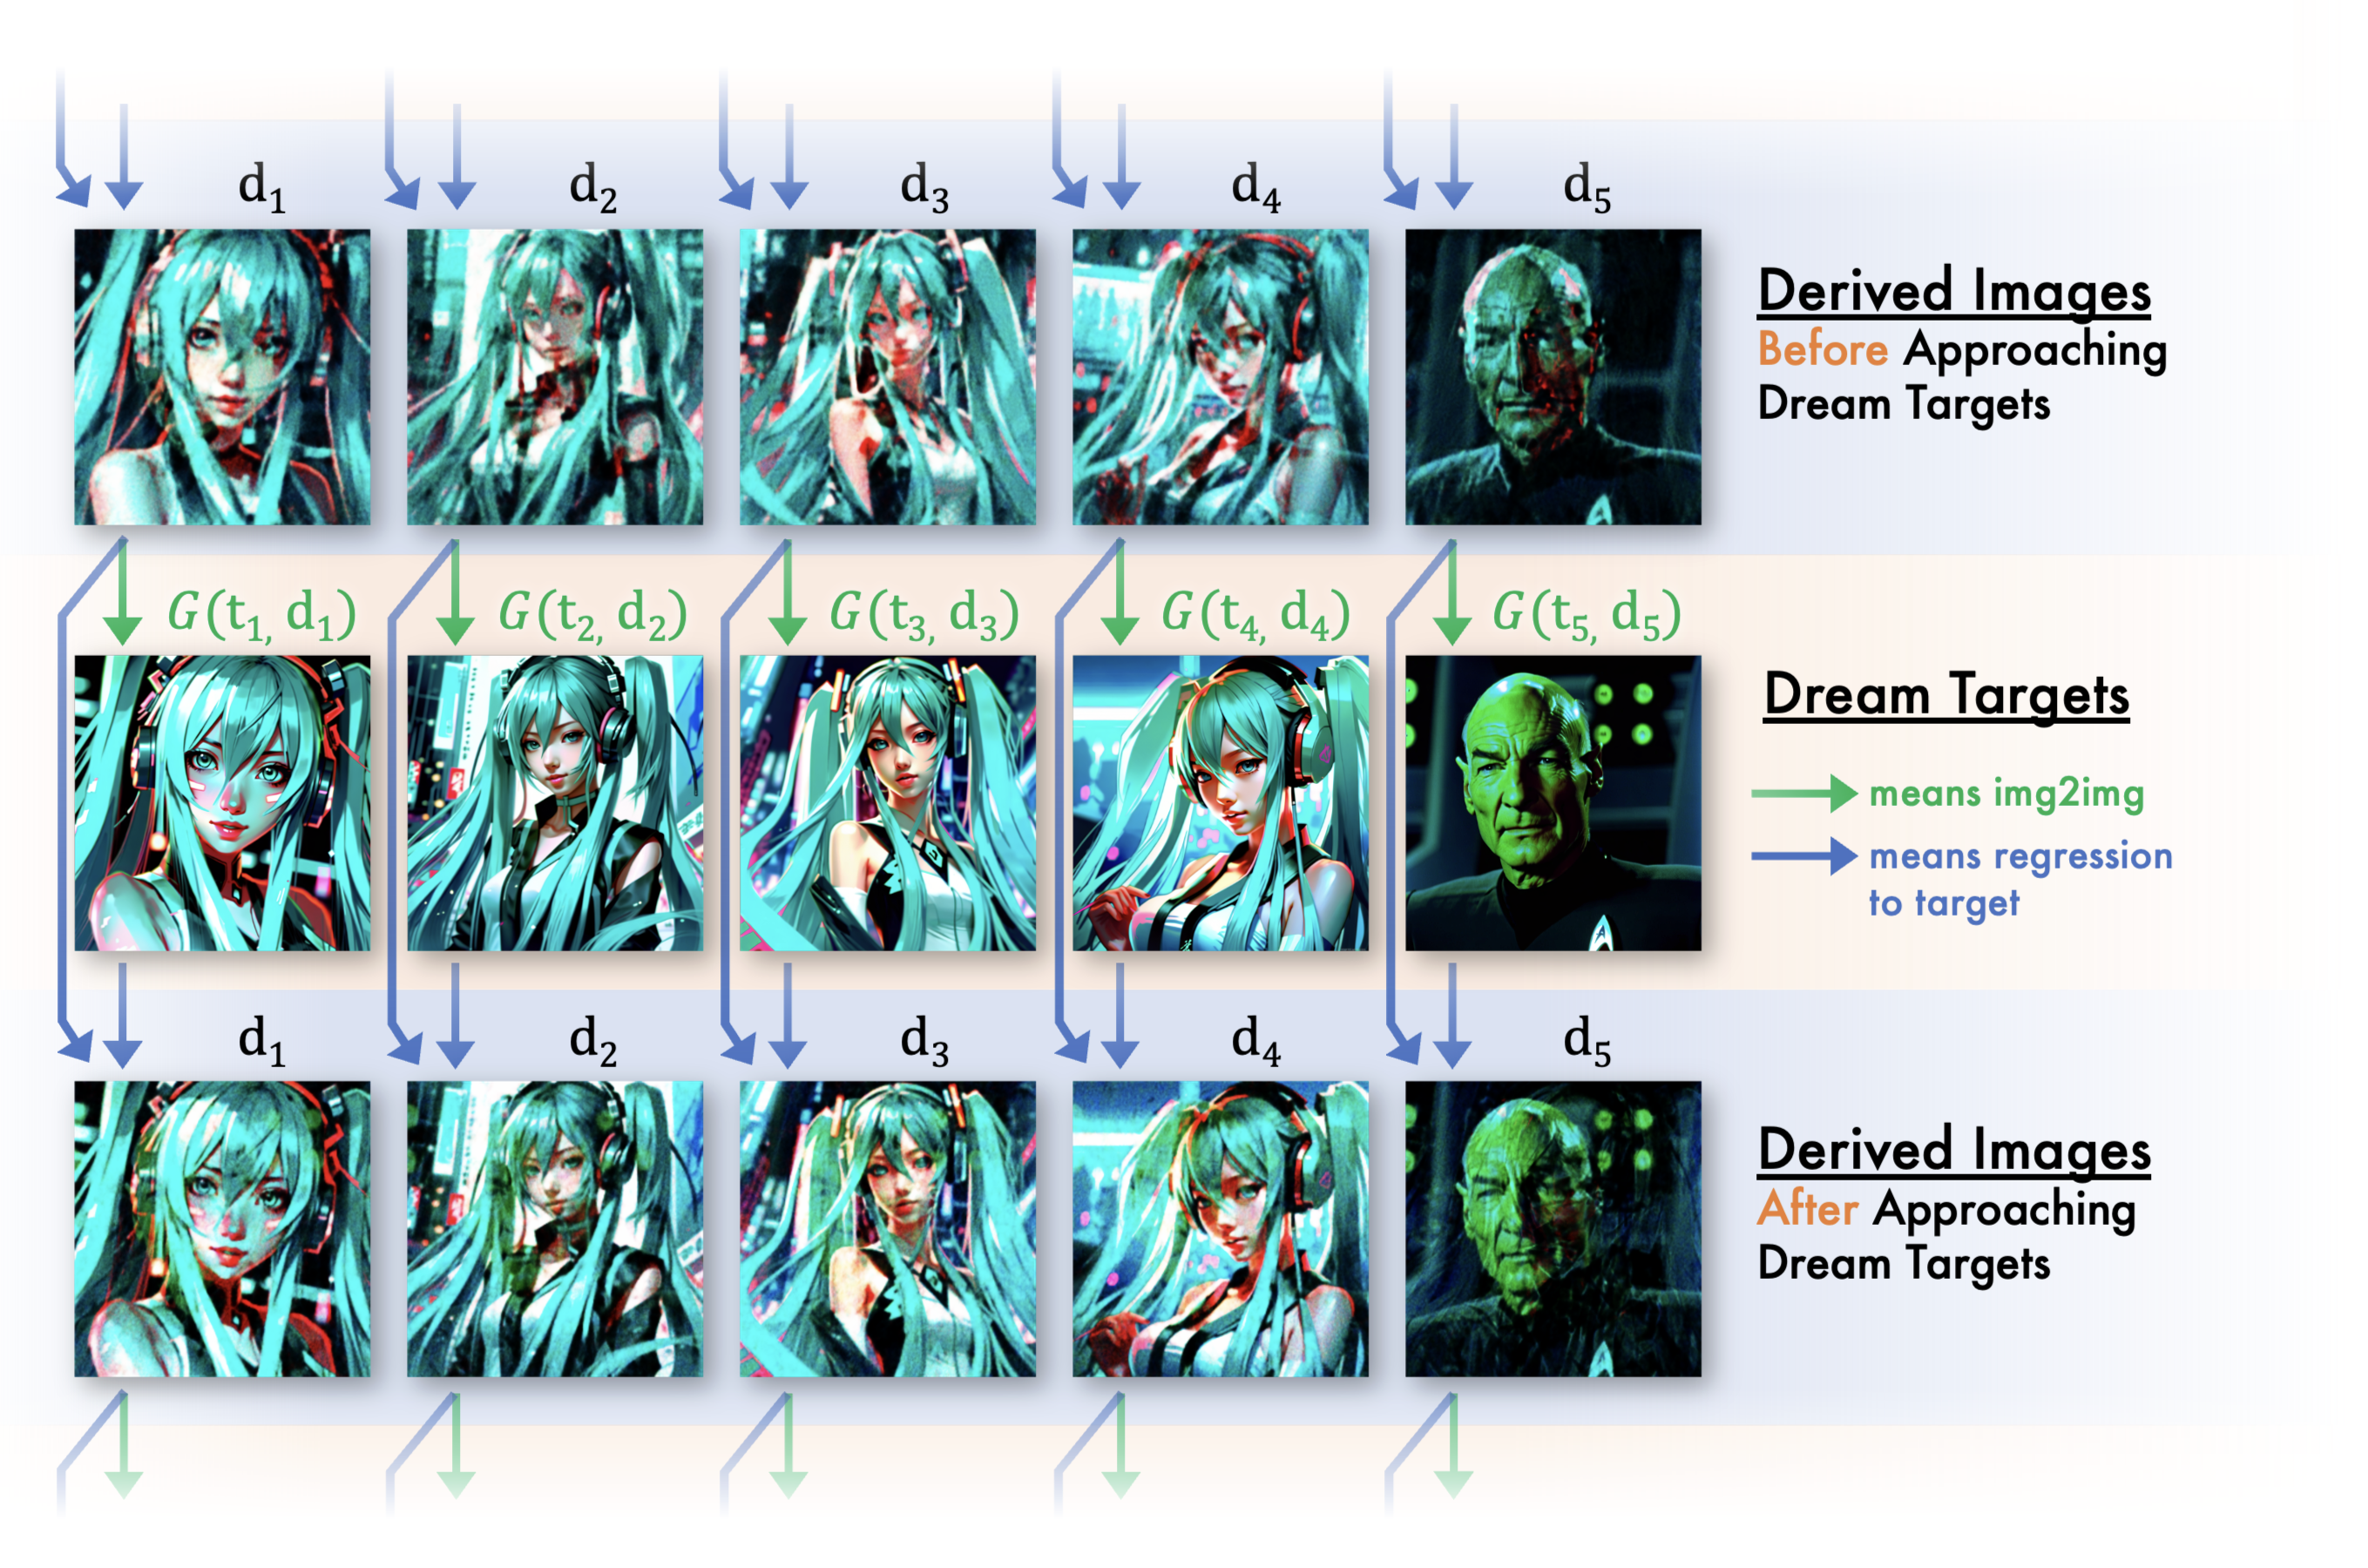
\includegraphics[width=\linewidth, trim={1cm 1cm 6cm 1cm}, clip]{src/2_DiffIllusions/figs/approaching_dreams.png}
  \caption[Dream Target Loss Illustration]{We depict the dream-target loss above. It is an iterative process, refining derived images using SDEdit to create target images, which the derived images are then regressed to with gradient descent. Note how the derived images look more like the targets after approaching them than before, such as the man's green face.}
  \label{diffill_fig:fig-dream-approach}
\end{figure}

Instead, Dream Target Loss ($\mathcal{L}^{\text{DT}}$) periodically applies a conditional image-to-image process $z_i = \mathcal{G}(t_i, d_i)$ to obtain a target image $z_i$ for each derived image $d_i$, conditioned on the textual prompt $t_i$.
Then we gradually pull each derived image $d_i$ towards its target image $z_i$ using a combination of the structural image similarity loss ($\mathcal{L}_{SSIM}$) and a pixel-wise mean squared error loss ($\mathcal{L}_{2}$).

Therein, we obtain a joint loss to similarly learn optimal prime images $p_i$ resulting in derived images aligned to each of our target concepts.
\begin{align}
    z_i &= \mathcal{G}(t_i, d_i)\\
    \mathcal{L}_i^{\text{DT}}(z_i, d_i) &= \mathcal{L}_{\text{SSIM}}(z_i, d_i) + \mathcal{L}_{2}(z_i, d_i)
    \label{diffill_eq:img_sim}
\end{align}

An additional feature of the Dream Target Loss relative to the SD variant is that it tends to introduce less noise.

The total dream target loss is a weighted average across all per derived image loss terms.
\begin{align}
    \mathcal{L}^{\text{DT}} = \sum w_i \mathcal{L}_i^{\text{DT}}
\end{align} where the loss terms are weighted by importance values $w_{1\dots m}$. By default, all $w_i=1$ except in the hidden overlay illusion where the hidden image is prioritized via $w_5=3$.

In practice, for each target image, we optimize the prime image for multiple (i.e. $1000$) steps using the dream target loss.
Then we repeat the process with the latest prime image so that the target image is updated towards the current derived image for faster convergence (Illustrated in \cref{diffill_fig:fig-dream-approach}).
We implement $\mathcal{G}$ using SDEdit~\cite{meng2022sdedit} where random noise is first added to the input image, and the noisy image is then iteratively denoised conditioned on the text prompt using a frozen diffusion model to generate an output image (see \cref{diffill_sec:pseudocode}).

Note that in both Score Distillation Loss and Dream Target Loss, we propagate gradients to the prime images, updating their parametric representation (i.e. the weights of the MLP Fourier Feature Networks $\theta$), and the diffusion model is kept frozen.

\subsubsection{Visual Prompt}
Optionally, one or more $t_i$ can be given as a specific target image instead of a text prompt --- letting users hide targets such as QR codes or blocks of text.
In that case, for both phases, the discrepancy between the derived image and the target image is measured using \cref{diffill_eq:img_sim}, providing gradients for the prime images.

\subsection{Fabrication}
The flip illusions are trivial to manufacture in real life and need only a printer. The hidden overlay and rotation overlay illusions are created by printing their prime images on overhead display sheets on a color laser printer, before being laminated to protect them from scratches.
With a strong enough backlight, the hidden overlays and rotation overlay illusions can be performed on regular pieces of paper as well.


\section{Experiments}
In this section, we evaluate our framework presenting qualitative visualizations and quantitative metrics.

\subsection{Qualitative Evaluation}
We illustrate randomly selected example outputs of our Diffusion Illusions framework. Visualizations for our three selected illusion styles, Flip Illusion, Rotation Overlay Illusion, and Hidden Overlay Illusion are presented in \cref{diffill_fig:galflip},
\cref{diffill_fig:galrot}, and \cref{diffill_fig:galhid} respectively.
For more interactive examples, please refer to the project website \url{https://diffusionillusions.com}

\begin{figure}
    \centering
    \includegraphics[width=.7\linewidth, trim={0 0 0 1cm}, clip]{src/2_DiffIllusions/figs/rearrangeFlipIllusion.pdf}
    \caption[Flip Illusion Examples]{\textbf{Flip Illusion Examples:} Please view these images upside-down as well as right-side-up to see two different subjects. Note: In this illusion, $d_1 = p_1$}
    \label{diffill_fig:galflip}
\end{figure}

\begin{figure}
    \centering
    \includegraphics[width=0.98\linewidth,trim={0cm 0cm 1cm 0cm}, clip]{src/2_DiffIllusions/figs/rotGal.pdf}
    \caption[Rotation Overlay Examples]{\textbf{Rotation Overlay Examples:} On the left are the two prime images $p_1$, $p_2$, and on the right are the four derived images $d_{1\dots 4}$ that are obtained by taking the product of the primes, simulation of them overlaid on a backlight.}
    \label{diffill_fig:galrot}
\end{figure}

\begin{figure}
    \centering
    \includegraphics[width=0.96\linewidth, trim={0 0.95cm 0 0}, clip]{src/2_DiffIllusions/figs/hiddenGal.pdf}
    \caption[Hidden Overlay Examples]{\textbf{Hidden Overlay Examples:} On the left are the four prime images $p_1$, $p_2$, $p_3$, $p_4$ and on the right is the derived image $d_5 = p_1 \cdot p_2 \cdot p_3 \cdot p_4$, which simulates overlaying them over a backlight. Note: In this illusion, $d_i = p_i$ for $i\in 1\dots 4$}
    \label{diffill_fig:galhid}
\end{figure}


\subsection{Quantitative Evaluation}
\label{diffill_sec:numbers}
Next, we quantitatively benchmark the Hidden Overlay Illusion generated by the variants of Diffusion Illusion in multiple aspects and demonstrate the generalization ability and robustness of the proposed framework. Please check \cref{diffill_sec:more_eval} as well for other illusions and more details.

\noindent\textbf{Image Generation Protocol} \quad We design a pipeline that constructs diverse textual prompts randomly and automatically.
The pipeline relies on two sets of textual prompts.
The first set $T^s$ is of sentences where each sentence describes a unique art style of an image and contains one \textit{subject} token representing the potential subject of the sentence.
The second set $T^o$ is of different subjects like `dog', `cat', `car', and so on.
When generating images with a specific style $t^s \in T^s$, we uniformly sample five unique subjects $t^o_i$ where $i \in\{1, \ldots, 5\}$ from $T^o$.
Then we substitute the \textit{subject} token in $t^s$ with $t^o_i$ to construct the textual prompt $t_i$.
Finally, $t_1, \ldots, t_5$ is used to guide the generation of derived images.

For a full evaluation, the whole pipeline is repeated for $N$ times per style $t^s$ to generate $N$ groups of illusion images.
In practice, we set $|T^s| = 4$, $T_o$ is the set of all object classes except `person' in PASCAL VOC~\cite{everingham2010pascal} ($|T^o|=19$), and $N=64$.
Please refer to \cref{diffill_sec:more_eval} for the complete list of subjects and styles.

\noindent\textbf{Evaluation Metrics} \quad Inspired by recent works on diffusion model evaluation~\cite{yeh2023navigating, lee2023holistic}, we measure the following properties of the derived images:

\begin{itemize}
    \item \textit{Controllability:} how well the generated images align with the textual prompts. For each generated image and its corresponding textual prompt, we measure the \textit{average cosine similarity} between the image embedding and the text embedding, extracted from a pretrained CLIP~\cite{radford2021learning} model.
    \item \textit{Diversity:} the variety of generated images conditioned on the same prompt. For images generated by the same textual prompt, we calculate two \textit{Venti scores}~\cite{friedman2022vendi} independently based on two visual embeddings: the \texttt{[CLS]} embeddings of DINOv2~\cite{oquab2023dinov2} and CLIP visual embeddings (see Appendix).
    \item \textit{Aesthetics:} the assessment of an image's visual appeal and artistic quality. For each image, we utilize AVA LAION-Aesthetics Predictor V2, which is pretrained on AVA~\cite{murray2012ava} dataset, to estimate an aesthetics score range from 0 to 10.
\end{itemize}

In addition, we study a new property~\textit{Independence} specifically for the illusion scenario.
Intuitively, each image is expected to stick to its corresponding textual prompt while not being distracted by other textual prompts in the same group.
Such property is named as \textit{Independence}, which is different from \textit{Controllability} because independence is designed to reflect not only the similarity between an image and its corresponding textual prompt but also the \textit{dissimilarity} between the image and the textual prompts for other images.
In other words, this property focuses on how well the prime images can `hide' the overlay image or how challenging it will be for people to infer the overlay image from a single prime image and vice versa.

\begin{itemize}
\item \emph{Independence Score:} Therefore, we propose a new metric Independence Score to reflect such property. Consider a set of $m$ derived images, denoted as $\{d_1, d_2, \ldots, d_m\}$, along with their corresponding textual prompts $\{t_1, t_2, \ldots, t_m\}$. Initially, we extract the visual embeddings $v_i=f_v(d_i)$ and text embeddings $e_j=f_t(t_j)$ using the visual encoder $f_v$ and the text encoder $f_t$ from a pretrained CLIP~\cite{radford2021learning} model respectively. Subsequently, we compute the cosine similarity $k_{ij}=\text{CosineSimilarity}(v_i, e_j)$ between any visual and text embeddings $v_i$ and $e_j$. The results are assembled into a matrix $K$, where $k_{ij}$ is put in the $i$-th row and $j$-th column. The Independence Score $S_\mathrm{IS}$ is calculated by the following equations.
\begin{align}
K_0 &= \mathrm{Softmax}(K / \tau, 0) \\
K_1 &= \mathrm{Softmax}(K / \tau, 1) \\
S_\mathrm{IS} & := \min(\mathrm{diag}(K_0) \cup \mathrm{diag}(K_1))
\end{align}
where $\tau=0.05$ is a temperature constant, $\text{Softmax}(\cdot, l)$ stands for softmax operation along $l$-th dimension and $\text{diag}(\cdot)$ presents a set of the diagonal elements of $(\cdot)$.
$S_\mathrm{IS}$ is designed to become higher when all images $d_i$ align best with their corresponding textual prompts compared with other textual prompts.
\end{itemize}

\noindent\textbf{Methods} \quad The baseline method of our experiments is a vanilla SDXL generating target images with corresponding textual prompts independently for one step using score distillation loss. We benchmark four variants of our methods named A, B, C, and D. Method C is our default method. It involves 500 steps of score distillation loss followed by 8 steps of dream target loss and applies relative weights [1,1,1,1,3] respectively - which prioritizes the quality-derived hidden image over its constituent primes. In addition, Method A uses Stable Diffusion 1.5 instead of SDXL, which is used by all other methods. Method B uses equal weights for all derived images, using weights [1,1,1,1,1] respectively. Lastly, method D uses 4000 steps of score distillation loss followed by 1 step of dream target loss for smoothness, to evaluate the ability of score distillation loss alone in this task.
For fairness, all methods were constrained to run in a 15-minute time window on a single NVIDIA A100 GPU.

\noindent\textbf{Results} \quad For all metrics, we report the score distributions achieved by our default method and the baseline in \cref{diffill_fig:big-baseline-fig}.
\begin{figure}[h]
  \centering
  \includegraphics[width=1\linewidth]{src/2_DiffIllusions/figs/fig-overall-baseline.pdf}
  \caption[Baseline Comparison Score Distributions]{Comparison of multiple score distributions. Refer to axes for metrics. Our framework clearly outperforms the baseline for all metrics except diversity (Vendi Score). We argue the additional constraints intrinsic to our task (of generating illusions) contributed to reduced diversity.}
  \label{diffill_fig:big-baseline-fig}
\end{figure}

Our method significantly outperforms the baseline in all metrics except the Vendi Score, which is expected because, for our method, there are more constraints from the derived images applied during the generation process.

The score distributions of four variants of our method are presented in \cref{diffill_fig:big-score-fig}. Each row of \cref{diffill_fig:big-score-fig} presents two metrics. The subfigures on the left-hand side show the overall performance of a specific method.
In general, all methods perform similarly well in terms of Controllability (Cosine Similarity) and Diversity (Vendi Score) (the first two rows in \cref{diffill_fig:big-score-fig}). Method C shows significant advantages in Aesthetics (Aesthetics Score) and Methods C and D achieve relatively higher Independence Score.

\begin{figure}[h]
  \centering
  \includegraphics[width=\linewidth]{src/2_DiffIllusions/figs/final-clip_score.png}
  \includegraphics[width=\linewidth]{src/2_DiffIllusions/figs/final-vendi_score_dino.png}
  \includegraphics[width=\linewidth]{src/2_DiffIllusions/figs/final-aesthetics_score.png}
  \includegraphics[width=\linewidth]{src/2_DiffIllusions/figs/final-rm.png}
  \caption[Score Distributions by Method and Style]{Score distributions over methods (left) and styles (right). A, B, C, D stands for four variants of our method. Results indicate the significance of prompts for illusion generation.}
  \label{diffill_fig:big-score-fig}
\end{figure}


A detailed look at different art styles is presented on the right-hand side of each row of \cref{diffill_fig:big-score-fig}, where different metrics respond diversely to different art styles.
Controllability (Cosine Similarity) prefers Style 3 and Style 4 while the Diversity (Vendi Score) prefers Style 2.
The Aesthetics Score and Independence Score are generally robust to the different styles.
However, the Aesthetics Score prefers Style 4 slightly more than Style 1.

In conclusion, the prompts used are far more important than the chosen implementation. There is no clear one-size-fits-all method indicated by our quantitative evaluations, however, we observe that depending on the art styles and subjects used, a different method will be optimal.
One should carefully pick up a method when generating illusions in a specific art style.
A further study on subjects is available in the Appendix.

\subsection{Discussions}
\label{diffill_sec:discussion}
In this section, we discuss several observations that may inspire future investigation.

\noindent\textit{Q1: Can Diffusion Illusion yield better images when running for a longer time?}

\noindent Yes. \cref{diffill_fig:fig-grad-increase} presents the trend of Controllability (Cosine Similarity) and Aesthetics (Aesthetics Score) as the images used in \cref{diffill_sec:numbers} are getting optimized.
The term `relative time' is employed to denote the progression of wall-clock time during the optimization process.
A relative time value of 0 means the beginning of optimization, whereas a value of 1 marks its conclusion.
\cref{diffill_fig:fig-grad-increase} reveals a notable trend: there is a consistent increase in metrics as the optimization process advances.
\begin{figure}[h]
  \centering
  \includegraphics[width=0.4\textwidth]{src/2_DiffIllusions/figs/final-grad.png}
  \caption[Optimization Convergence]{CLIP Cosine Similarity (left) and Aesthetics Score (right) increase when optimizing for a longer time.}
  \label{diffill_fig:fig-grad-increase}
\end{figure}

\noindent\textit{Q2: Is Independence Score a qualitatively valid metric?}

\noindent Generally yes. \cref{diffill_fig:fig-sis} shows four illusions randomly selected with diverse independence scores. For each row, the subject of each image is listed above, and the method, style, and independence scores are listed on the left-hand side.
The four images grouped in the middle are prime images and they derive the overlay image on the right-hand side.
For the first two examples where the independence score is relatively high, each image aligns with its corresponding textual prompt.
However, for the third example, the overlay image is not closely related to the subject `sofa', resulting in a lower independence score.
Furthermore, in the last example of \cref{diffill_fig:fig-sis}, the overlay image visually biases more towards `cow' instead of `bottle', leading to the lowest independence score.

\begin{figure}[h]
  \centering
  \includegraphics[width=\linewidth]{src/2_DiffIllusions/figs/sis_large_demo.jpg}
  \caption[Independence Score Examples]{Examples with diverse independence scores}
  \label{diffill_fig:fig-sis}
\end{figure}

\noindent\textit{Q3: What are the reasons to use Fourier Features Network?}

\noindent Earlier experiments optimizing prime images directly in pixel space resulted in information being encoded at very high frequencies and requiring pixel-perfect alignment to generate the intended derived images (see \cref{diffill_fig:fig-noisy}). While the result was pleasing when viewed digitally, it was impractical for real-world illusions. Motivated by previous arguments \cite{Burgert2022PeekabooTT, Burgert2022}, we elect to use Fourier Features Network \cite{tancik2020fourier} based parametric image representations.

\begin{figure}[h]
  \centering
  \includegraphics[width=\linewidth]{src/2_DiffIllusions/figs/demo_noisy_fft.jpg}
  \caption[Pixel-Space Optimization Artifacts]{A Hidden Overlay image with prime images optimized directly in pixel space. While high-frequency encoding of the hidden image results in less perceivable interference in each individual image, it results in a brittle illusion that is disrupted without pixel-perfect printing and alignment.}
  \label{diffill_fig:fig-noisy}
\end{figure}



\section{Conclusion}
In this paper, we establish the formal definition of the problem of generating illusions and introduce Diffusion Illusions, a versatile pipeline designed for the generation of a diverse array of illusions.
Complemented by comprehensive experiments conducted across multiple facets, we verify the effectiveness of our proposed method qualitatively and quantitatively.
We also successfully fabricate the prime images in the real world.
Other areas to explore include more types of illusion generation and creative ways to take advantage of diffusion models.

\paragraph{Limitations}
The main limitation of our framework is the relatively high inference time required for generating illusions. While our framework improves over plain score distillation in terms of inference time, we are still slow. Improving the speed of illusion generation frameworks such as ours presents an interesting future direction.
We note that contemporary work has already explored ways to minimize this inference time.

Furthermore,
the effectiveness of visual illusion in the real world may vary a lot due to the errors introduced in the printing process. \cref{diffill_fig:simreal2} and \cref{diffill_fig:simreal} present the effect of the color shifts when printing the images.

\begin{figure}[t]
  \centering
  \includegraphics[width=1\linewidth, trim={1cm 1cm 1cm 1cm}, clip]{src/2_DiffIllusions/figs/SimRealRot.jpg}
  \caption[Rotation Overlay Simulation vs.\ Reality]{The colors shift after printing out Rotation Overlay Illusion images. First row: digital copy of the images and the overlay simulation. Second row: real-world photos of the printed images.}
  \label{diffill_fig:simreal2}
\end{figure}

\begin{figure}[t]
  \centering
  \includegraphics[width=1\linewidth]{src/2_DiffIllusions/figs/SimRealHidAdjust.jpg}
  \caption[Hidden Overlay Simulation vs.\ Reality]{The colors shift after printing out Hidden Overlay Illusion images. First row: digital copy of the images and the overlay simulation. Second row: real-world photos of the printed images.}
  \label{diffill_fig:simreal}
\end{figure}

Other limitations include biases contained in our models (discussed in detail under the ethics statement).

\paragraph{Reproducibility Statement}
Our work builds off open-source models whose pre-trained weights are publicly available. Our framework simply performs inference time optimizations to generate illusions. In our paper, we detail all specifics of our implementation (including PyTorch style pseudo-code) necessary to generate such illusions. Our code (and all material necessary to replicate results in paper) will be released publicly.

\paragraph{Ethics Statement}
A main ethical concern for any generative art model is that it will reduce the demand for human artists in its domain. Generating optical illusion artwork is a very difficult artistic task, and there are few artists that attempt it. Thus, the genre of illusions is currently relatively small and there is limited demand for illusions at present. Diffusion Illusions makes the generation of optical illusions accessible to the general public, making illusions more accessible to the layperson. We believe that, if anything, Diffusion Illusions and related works are likely to increase interest in illusions and the demand for human-created illusions as a result.
Secondly, our experiments utilize Stable Diffusion 1.5 and Stable Diffusion-XL models, and thus our reference implementation of the Diffusion Illusions pipeline will replicate any biases contained within these models. These models are trained on the LAION-2B(en) and LAION-5B datasets, and may over-represent English-language or Western content. The Stable Diffusion 1.5 and Stable Diffusion-XL models are intended for research purposes only, and thus our reference implementation should also be used exclusively for research and informative purposes. Some recent models, including DeepFloyd, are licensed for limited production use and our pipeline easily generalizes to them; however, they have higher system requirements.

\paragraph{Contributions}
RB led the project, conceived the prime image / derived image illusion relationship, invented the classes of hidden and rotation overlay illusions, and designed \& implemented the Diffusion Illusions pipeline.
XL designed and performed all quantitative evaluation experiments.
AL formalized and wrote the Illusion problem statement and contributed to paper writing.
KR discussed multiple aspects of the project, supported designing a prior framework (Peekaboo~\cite{Burgert2022PeekabooTT}) important for building our setup, and contributed to paper writing.
MR supervised the project, advised on research direction, and discussed all aspects of the project.

\paragraph{Acknowledgements}
We would like to thank Brian Price and Jinghuan Shang for helpful discussions about this paper, and Jongwoo Park for both his discussions as well as posing for the flip illusion photo in \cref{diffill_fig:teaser}. This material is based upon work supported by the National Science Foundation Graduate Research Fellowship under Grant No. 2234683.
